\begin{framed}

Objetivos:
\begin{itemize}
    \item Encontrar la relación entre variables termodinámicas de un flujo isentrópico de un gas ideal y sus condiciones de estancamiento.
    \item Estudiar la forma de obtener un flujo supersónico desde una tobera.
    \item Describir el flujo compresible en una tobera convergente-divergente.
\end{itemize}

Contenidos:
\begin{itemize}
    \item Flujo isentrópico de gas ideal y sus condiciones al estancamiento. 
    \item Flujo en una tobera convergente y divergente en el caso subsónico y supersónico. 
    \item Condiciones críticas y flujo ahogado.
    \item La tobera convergente-divergente.
\end{itemize}

Bibliografía:
\begin{itemize}
    \item Fox, R. W., Pritchard, P. J. y McDonald, A. T. (2009) Introduction to Fluid Mechanics. John Wiley \& Sons. Sección 12.3-13.2.
\end{itemize}
\end{framed}

\section*{Flujo isentrópico de un gas ideal}

En la clase pasada repasamos conceptos de termodinámica, y llegamos a diferentes expresiones relacionando presión, temperatura y densidad para procesos isentrópicos de gases ideales. 
Ahora, analizaremos un flujo isentrópico de gas ideal, para poder encontrar ecuaciones que relacionen un estado termodinámico con las condiciones del flujo al estancamiento.
Poder saber las condiciones termodinámicas de un flujo respecto a su estado de estancamiento es de gran utilidad para aplicaciones, ya que conociendo las condiciones del gas en un estanque (donde está quieto), podemos predecir su estado, por ejemplo, a lo largo de una tobera.

Analicemos un flujo isentrópico de un gas ideal que va desacelerándose hasta llegar a velocidad 0 (estancamiento), usando un tubo de corriente de ancho $dx$ como volumen de control (Figura \ref{fig:volumen_control}).
%
\begin{figure}
\centering
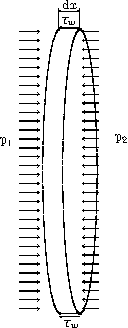
\includegraphics[width=0.7\textwidth]{clase14/volumen_control.pdf}
\caption{Volumen de control sobre línea de corriente que llega a la condición de estancamiento}
\label{fig:volumen_control}
\end{figure}
%
El volumen de control se encuentra en un punto genérico $x$, donde la velocidad del flujo es $V$, densidad $\rho$, presión $p$, temperatura $T$ y el tubo de corriente tiene area $A$. 
Después del volumen de control, estas condiciones cambian a $V+dV$, $\rho+d\rho$, $p+dp$, $T+dT$ y $A+dA$.
Aguas abajo, el flujo de desacelera a velocidad $V=0$, y encontramos las condiciones de estancamiento $\rho_0$, $p_0$ y $T_0$.

Partamos por analizar continuidad sobre el solumen de control.
Ya que es un tubo de corriente, no hay flujo a través del ``manto'' del columen de control, si no que solamente por las secciones transversales.
Digamos que la velocidad y densidad son constantes en cada sección transversal (lo cual no es una mala aproximación si consideramos un $A$ pequeño).
En estado estacionario (sin acumulación), la conservación de masa nos lleva a
%
\begin{equation}\label{eq:continuidad_isentropico}
\rho VA = (\rho+d\rho)(V+dV)(A+dA)
\end{equation}

El análisis de cantidad de movimiento es un poco más engorroso.
De Mecánica de Fluidos General, sabemos que si no hay acumulación, el teorema de transporte de Reynolds en conjunto con la segunda ley de Newton da:
%
\begin{equation}\label{eq:momentum_isentropico}
\sum \mathbf{F} = \oint_S \mathbf{V} \rho \mathbf{V}\cdot\mathbf{n} dS.
\end{equation}

Partamos con la suma de fuerzas en el eje $x$.
Usando la Figura \ref{fig:cantidad_mov} como referencia, en las caras transversales tenemos una fuerza $pA$ por el lado izquierdo y $(p+dp)(A+dA)$ por el derecho.
Por otra parte, el manto tiene una forma arbitraria, y una distribución de presión sobre ésta tiene una componente en el eje $x$.
Considerando que $dx$ es pequeño, asumamos que la fuerza generada por la presión sobre este manto es igual al promedio entre la presión antes y después del volumen de control, es decir $\overline{p} = p+dp/2$.
Entonces, la fuerza sobre el manto es $(p+dp/2)S$, donde $S$ es el área del manto, y $S=Ld$ donde $L$ es el perímetro y $d$ el ancho ($dx=d\cos\alpha$) .
Nosotros estamos interesados en la componente $x$ de la fuerza, que es $(p+dp/2)Ld\sin\alpha$, pero $d\sin\alpha$ es la proyección de $d$ en el eje $y$, y multiplicado por el perímetro $L$, no es más de la diferencia entre las áreas de entrada y salida del volumen de control ($dA$).
De esta forma, podemos escribir la componente $x$ de la fuerza sobre el manto como $(p+dp/2)dA$, y despreciando los términos con diferenciales de orden mayor a 1, la suma de fuerza queda
%
\begin{equation}
\sum F_x = pA - (p+dp)(A+dA) + (p+dp/2)dA = -dpA
\end{equation}
%
\begin{figure}
\centering
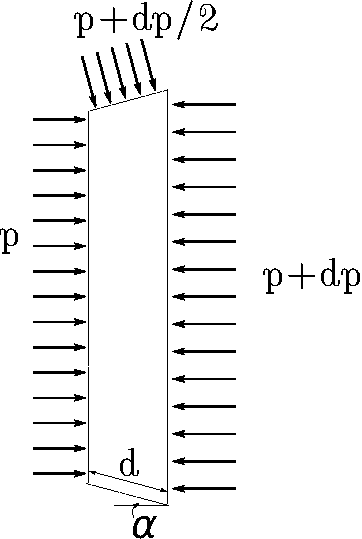
\includegraphics[width=0.4\textwidth]{clase14/cantidad_mov.pdf}
\caption{Análisis de cantidad de movimiento sobre volumen de control.}
\label{fig:volumen_control}
\end{figure}

Conociendo la suma de fueras, y asumiendo que la variables son constantes en la sección transversal, podemos reescribir la Ec. \eqref{eq:momentum_isentropico} como
%
\begin{align}
-dpA &= -V\rho VA + (V+dV)\underbrace{(\rho+d\rho)(V+dV)(A+dA)}_{=\rho VA\text{ por continuidad (Ec.\eqref{eq:continuidad_isentropico})}}\nonumber\\
\Rightarrow -dp &= \rho V(-V+V+dV)\nonumber\\
-dp &= \rho VdV\nonumber\\
\frac{dp}{\rho} &+ d\left(\frac{V^2}{2}\right) = 0
\end{align}
